


\begin{frame}{Evoluci\'on de las tecnolog\'ias de la informaci\'on}

    \begin{overlayarea}{\linewidth}{\textheight}
        \vspace{10mm}
        \centering
    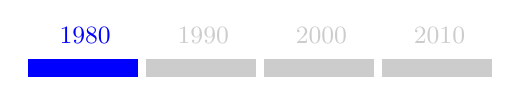
\begin{tikzpicture}[xscale=0.15]

        \node[rectangle, fill=blue, minimum width=14mm] at (0,0) {};
        \node[anchor=south, color=blue, inner sep=0pt] at (0.2,0.3) {\small 1980};

        \node[rectangle, fill=black!20, minimum width=14mm] at (10,0) {};
        \node[anchor=south, color=black!20, inner sep=0pt] at (10.2,0.3) {\small 1990};

        \node[rectangle, fill=black!20, minimum width=14mm] at (20,0) {};
        \node[anchor=south, color=black!20, inner sep=0pt] at (20.2,0.3) {\small 2000};

        \node[rectangle, fill=black!20, minimum width=14mm] at (30,0) {};
        \node[anchor=south, color=black!20, inner sep=0pt] at (30.2,0.3) {\small 2010};
    \end{tikzpicture}

    \vspace{20pt}

    \begin{columns}[T]
        \begin{column}{0.23\textwidth}
            \centering
            \includegraphics[width=1.3cm]{img/sqldb_nb.png}\\
            Primeros sistemas gestores de bases de datos relacionales comerciales
        \end{column}
        \begin{column}{0.23\textwidth}
            \centering
            \includegraphics[width=1.3cm]{img/sql.png}\\
            Est\'andar de lenguaje SQL
        \end{column}

        \begin{column}{0.23\textwidth}
            \centering
            \includegraphics[width=1.3cm]{img/server.png}\\
            {Primeros servidores de bases de datos relacionales}
        \end{column}
        \begin{column}{0.23\textwidth}
            \centering
            \includegraphics[width=1.3cm]{img/monitor.png}\\
            Procesamiento anal\'itico de datos
        \end{column}
    \end{columns}
    \end{overlayarea}
   

\end{frame}



\begin{frame}{Evoluci\'on de las tecnolog\'ias de la informaci\'on}
    \begin{overlayarea}{\textwidth}{\textheight}
        \vspace{10mm}
    \centering
    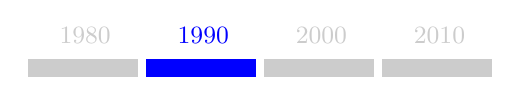
\begin{tikzpicture}[xscale=0.15]

        \node[rectangle, fill=black!20, minimum width=14mm] at (0,0) {};
        \node[anchor=south, color=black!20, inner sep=0pt] at (0.2,0.3) {\small 1980};

        \node[rectangle, fill=blue, minimum width=14mm] at (10,0) {};
        \node[anchor=south, color=blue, inner sep=0pt] at (10.2,0.3) {\small 1990};

        \node[rectangle, fill=black!20, minimum width=14mm] at (20,0) {};
        \node[anchor=south, color=black!20, inner sep=0pt] at (20.2,0.3) {\small 2000};

        \node[rectangle, fill=black!20, minimum width=14mm] at (30,0) {};
        \node[anchor=south, color=black!20, inner sep=0pt] at (30.2,0.3) {\small 2010};
    \end{tikzpicture}

    \vspace{20pt}

    \begin{columns}[T]
        \begin{column}{0.23\textwidth}
            \centering
            \includegraphics[width=1.3cm]{img/website.png}\\
            Internet
        \end{column}
        \begin{column}{0.23\textwidth}
            \centering
            \includegraphics[width=1.3cm]{img/online-store.png}\\
            Negocios online
        \end{column}

        \begin{column}{0.23\textwidth}
            \centering
            \includegraphics[width=1.3cm]{img/xml.png}\\
            Modelo orientado a objetos\\ XML
        \end{column}
    \end{columns}
\end{overlayarea}

\end{frame}


\begin{frame}{Evoluci\'on de las tecnolog\'ias de la informaci\'on}
    \begin{overlayarea}{\textwidth}{\textheight}
        \vspace{10mm}
    \centering
    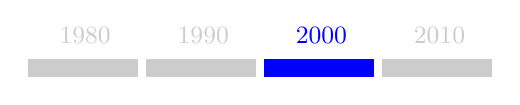
\begin{tikzpicture}[xscale=0.15]

        \node[rectangle, fill=black!20, minimum width=14mm] at (0,0) {};
        \node[anchor=south, color=black!20, inner sep=0pt] at (0.2,0.3) {\small 1980};

        \node[rectangle, fill=black!20, minimum width=14mm] at (10,0) {};
        \node[anchor=south, color=black!20, inner sep=0pt] at (10.2,0.3) {\small 1990};

        \node[rectangle, fill=blue, minimum width=14mm] at (20,0) {};
        \node[anchor=south, color=blue, inner sep=0pt] at (20.2,0.3) {\small 2000};

        \node[rectangle, fill=black!20, minimum width=14mm] at (30,0) {};
        \node[anchor=south, color=black!20, inner sep=0pt] at (30.2,0.3) {\small 2010};
    \end{tikzpicture}

    \vspace{20pt}

    \begin{columns}[T]
        \begin{column}{0.23\textwidth}
            \centering
            \includegraphics[width=1.3cm]{img/warehouse.png}\\
            Data Warehousing
        \end{column}

        \begin{column}{0.23\textwidth}
            \centering
            \includegraphics[width=1.3cm]{img/networking.png}\\
            Redes sociales
        \end{column}
        \begin{column}{0.23\textwidth}
            \centering
            \includegraphics[width=1.3cm]{img/booking.png}\\
            Computaci\'on m\'ovil
        \end{column}

        \begin{column}{0.23\textwidth}
            \centering
            \includegraphics[width=1.3cm]{img/big-data.png}\\
            Inicios del Big Data
        \end{column}

    \end{columns}
\end{overlayarea}

\end{frame}



\begin{frame}{Evoluci\'on de las tecnolog\'ias de la informaci\'on}
    \begin{overlayarea}{\textwidth}{\textheight}
        \vspace{10mm}
    \centering
    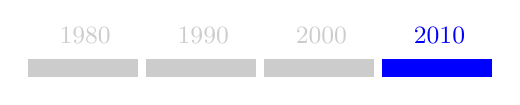
\begin{tikzpicture}[xscale=0.15]

        \node[rectangle, fill=black!20, minimum width=14mm] at (0,0) {};
        \node[anchor=south, color=black!20, inner sep=0pt] at (0.2,0.3) {\small 1980};

        \node[rectangle, fill=black!20, minimum width=14mm] at (10,0) {};
        \node[anchor=south, color=black!20, inner sep=0pt] at (10.2,0.3) {\small 1990};

        \node[rectangle, fill=black!20, minimum width=14mm] at (20,0) {};
        \node[anchor=south, color=black!20, inner sep=0pt] at (20.2,0.3) {\small 2000};

        \node[rectangle, fill=blue, minimum width=14mm] at (30,0) {};
        \node[anchor=south, color=blue, inner sep=0pt] at (30.2,0.3) {\small 2010};
    \end{tikzpicture}

    \vspace{20pt}

    \begin{columns}[T]
        
        \begin{column}{0.23\textwidth}
            \centering
            \includegraphics[width=1.6cm]{img/noSQL.png}\\
            Sistemas gestores de bases de datos NoSQL
        \end{column}

        \begin{column}{0.23\textwidth}
            \centering
            \includegraphics[width=1.3cm]{img/cloud-computing.png}\\
            Computaci\'on en la nube
        \end{column}
    \end{columns}
\end{overlayarea}

\end{frame}